\documentclass{article}
\usepackage{amsmath}
\usepackage{tikz}

\begin{document}

The partition, $\sum\limits_{k=1}^R (\beta_k + m_{k-1} + 1)(R - k + 1) - R$.

\begin{center}
    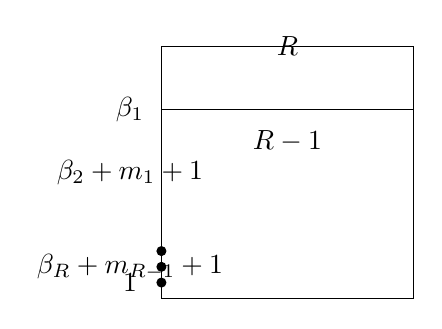
\begin{tikzpicture}[scale=0.8]
        % Draw the rectangle
        \draw (0,0) rectangle (4,4);
        
        % Label the top of the rectangle
        \node at (2,4) {$R$};
        
        % Draw the horizontal line
        \draw (0,3) -- (4,3);
        
        % Label the horizontal line
        \node at (2,2.5) {$R-1$};
        
        % Draw the vertical lines
        \draw (0,2) -- (0,0);
        \draw (0,1) -- (0,0);
        \draw (0,0.5) -- (0,0);
        \draw (0,0.25) -- (0,0);
        
        % Label the vertical lines
        \node at (-0.5,3) {$\beta_1$};
        \node at (-0.5,2) {$\beta_2 + m_1 + 1$};
        \node at (-0.5,0.5) {$\beta_R + m_{R-1} + 1$};
        \node at (-0.5,0.25) {$1$};
        
        % Draw the dots
        \filldraw[black] (0,0.75) circle (2pt);
        \filldraw[black] (0,0.5) circle (2pt);
        \filldraw[black] (0,0.25) circle (2pt);
    \end{tikzpicture}
\end{center}

\end{document}